\newcommand{\dropperTagResultsAucTable}{
    \begin{table}[H]
        \centering
        \begin{tabular}{|p{2,8cm}||P{2,4cm} P{2,4cm} P{2,4cm}|}
            \hline
            Dropper Tag & ALOHA\newline (M/B only) & ALOHA & Proposed\newline Model \\
            \hline
            AUC-ROC & - & 0.973$\pm$0.001 & \textBF{0.979$\pm$0.000} \\
            \hline
        \end{tabular}
        \caption[Dropper Tag prediction task AUC-ROC results]{AUC-ROC (Area Under Curve) of the different models for the \textbf{Dropper Tag} prediction task. Results were aggregated over \textBF{2} training runs with different weight initializations and minibatch orderings. Best results are shown in \textbf{bold}.} \label{tab:dropperTag_auc}
    \end{table}
}

\newcommand{\dropperTagResultsAtFprTable}{
    \begin{center}
        \begin{longtable}[c]{|P{3,2cm}||P{1,8cm} P{1,8cm} P{1,8cm} P{1,8cm} P{1,8cm}|}
            \hline
            Dropper Tag & \multicolumn{5}{c|}{{FPR}} \\
            & $10^{-5}$ & $10^{-4}$ & $10^{-3}$ & $10^{-2}$ & $10^{-1}$ \\
            \hline
            \endfirsthead

            \caption*{\raggedright ...continued from previous page} \\
            \hline
            Dropper Tag & \multicolumn{5}{c|}{\textbf{FPR}} \\
            & $10^{-5}$ & $10^{-4}$ & $10^{-3}$ & $10^{-2}$ & $10^{-1}$ \\
            \hline
            \endhead

            \caption*{\raggedleft ...continued on next page} \\
            \endfoot

            \caption[Dropper Tag prediction task results]{Mean and standard deviation results (TPR, Accuracy, Recall, Precision and F1-Score) of the different models for the \textbf{Dropper Tag} prediction task at different \textbf{FPR}s (\textit{False Positive Rates}). Results were aggregated over \textBF{2} training runs with different weight initializations and minibatch orderings. Best results are shown in \textbf{bold}. Under \textbf{TPR} results are also presented the percentage reduction in mean detection error and in ROC curve standard deviation introduced by the \textit{Proposed Model} with respect to both \textit{ALOHA} model and \textit{Joint Embedding}.} \label{tab:dropperTag_results_at_fpr} \\
            \endlastfoot

            \multicolumn{6}{|c|}{\textbf{TPR}} \\
            \hline
            ALOHA (M/B only) & - & - & - & - & - \\
            ALOHA & 0.051$\pm$0.024 & 0.053$\pm$0.023 & 0.069$\pm$0.021 & 0.663$\pm$0.045 & 0.920$\pm$0.004 \\
            Proposed Model & 0.045$\pm$0.020 & 0.053$\pm$0.019 & 0.069$\pm$0.017 & 0.729$\pm$0.013 & \textBF{0.950$\pm$0.007} \\
            \hline
            Error Reduction wrt\newline ALOHA (M/B only) & - & - & - & - & - \\
            Error Reduction wrt\newline ALOHA & -0.6\% & 0.0\% & 0.0\% & 19.6\% & 37.5\% \\
            \hline
            Std Reduction wrt\newline ALOHA (M/B only) & - & - & - & - & - \\
            Std Reduction wrt\newline ALOHA & 16.7\% & 17.4\% & 19.0\% & 71.1\% & -75.0\% \\
            \hline
            \multicolumn{6}{|c|}{\textbf{Accuracy}} \\
            \hline
            ALOHA (M/B only) & - & - & - & - & - \\
            ALOHA & 0.879$\pm$0.003 & 0.879$\pm$0.003 & 0.880$\pm$0.003 & 0.948$\pm$0.006 & 0.903$\pm$0.001 \\
            Proposed Model & 0.878$\pm$0.003 & 0.879$\pm$0.002 & 0.880$\pm$0.002 & \textBF{0.957$\pm$0.002} & \textBF{0.906$\pm$0.001} \\
            \hline
            \multicolumn{6}{|c|}{\textbf{Recall}} \\
            \hline
            ALOHA (M/B only) & - & - & - & - & - \\
            ALOHA & 0.051$\pm$0.024 & 0.053$\pm$0.023 & 0.069$\pm$0.021 & 0.663$\pm$0.045 & 0.920$\pm$0.004 \\
            Proposed Model & 0.045$\pm$0.020 & 0.053$\pm$0.019 & 0.069$\pm$0.017 & 0.729$\pm$0.013 & \textBF{0.950$\pm$0.007} \\
            \hline
            \multicolumn{6}{|c|}{\textbf{Precision}} \\
            \hline
            ALOHA (M/B only) & - & - & - & - & - \\
            ALOHA & \textBF{0.999$\pm$0.000} & 0.985$\pm$0.007 & 0.902$\pm$0.028 & 0.906$\pm$0.006 & 0.574$\pm$0.001 \\
            Proposed Model & 0.998$\pm$0.001 & 0.986$\pm$0.005 & 0.905$\pm$0.021 & 0.914$\pm$0.001 & \textBF{0.582$\pm$0.002} \\
            \hline
            \multicolumn{6}{|c|}{\textbf{F1 Score}} \\
            \hline
            ALOHA (M/B only) & - & - & - & - & - \\
            ALOHA & 0.096$\pm$0.043 & 0.099$\pm$0.042 & 0.127$\pm$0.037 & 0.765$\pm$0.032 & 0.707$\pm$0.002 \\
            Proposed Model & 0.085$\pm$0.036 & 0.101$\pm$0.034 & 0.128$\pm$0.030 & 0.811$\pm$0.008 & \textBF{0.722$\pm$0.003} \\
            \hline
        \end{longtable}
    \end{center}
}

\newcommand{\dropperTagResultsSummaryTable}{
    \begin{table}[H]
        \centering
        \begin{tabular}{|P{3,2cm}||P{1,8cm} P{1,8cm} P{1,8cm} P{1,8cm} P{1,8cm}|}
            \hline
            \multicolumn{6}{|c|}{Dropper Tag (at FPR $=1\%$)} \\
            \hline
            Model & TPR & Accuracy & Precision & Recall & F1 score \\
            \hline
            ALOHA (M/B only) & - & - & - & - & - \\
            ALOHA & 0.663$\pm$0.045 & 0.948$\pm$0.006 & 0.906$\pm$0.006 & 0.663$\pm$0.045 & 0.765$\pm$0.032 \\
            Proposed Model & 0.729$\pm$0.013 & \textBF{0.957$\pm$0.002} & 0.914$\pm$0.001 & 0.729$\pm$0.013 & 0.811$\pm$0.008 \\
            \hline
        \end{tabular}
        \caption[Summary of Dropper Tag prediction task results]{Summary of the mean and standard deviation results of the different models for the \textbf{Dropper Tag} prediction task at \textbf{FPR} $=1\%$. Results were aggregated over \textBF{2} training runs with different weight initializations and minibatch orderings. Best results are shown in \textbf{bold}.} \label{tab:dropperTag_result_summary}
    \end{table}
}

\newcommand{\dropperTagRocAlohaMB}{
    \begin{figure}[H]
        \vspace*{-0.5cm}
        \centering
        \includegraphics[width=0.6\textwidth]{./results/dropper_tag_roc_alohaMB.png}
        \vspace*{-0.2cm}
        \caption[Dropper Tag prediction task ALOHA (M/B only) ROC curve]{ROC curve and AUC statistics of \textBF{ALOHA (M/B only)} model for the \textbf{Dropper Tag}. The line represents the \textit{mean} TPR at a given FPR, while the shaded region represents the \textit{standard deviation}. Statistics were computed over \textBF{2} training runs, each with random parameter initialization.}
        \label{fig:dropperTagRocAlohaMB}
    \end{figure}
}

\newcommand{\dropperTagRocAloha}{
    \begin{figure}[H]
        \vspace*{-0.5cm}
        \centering
        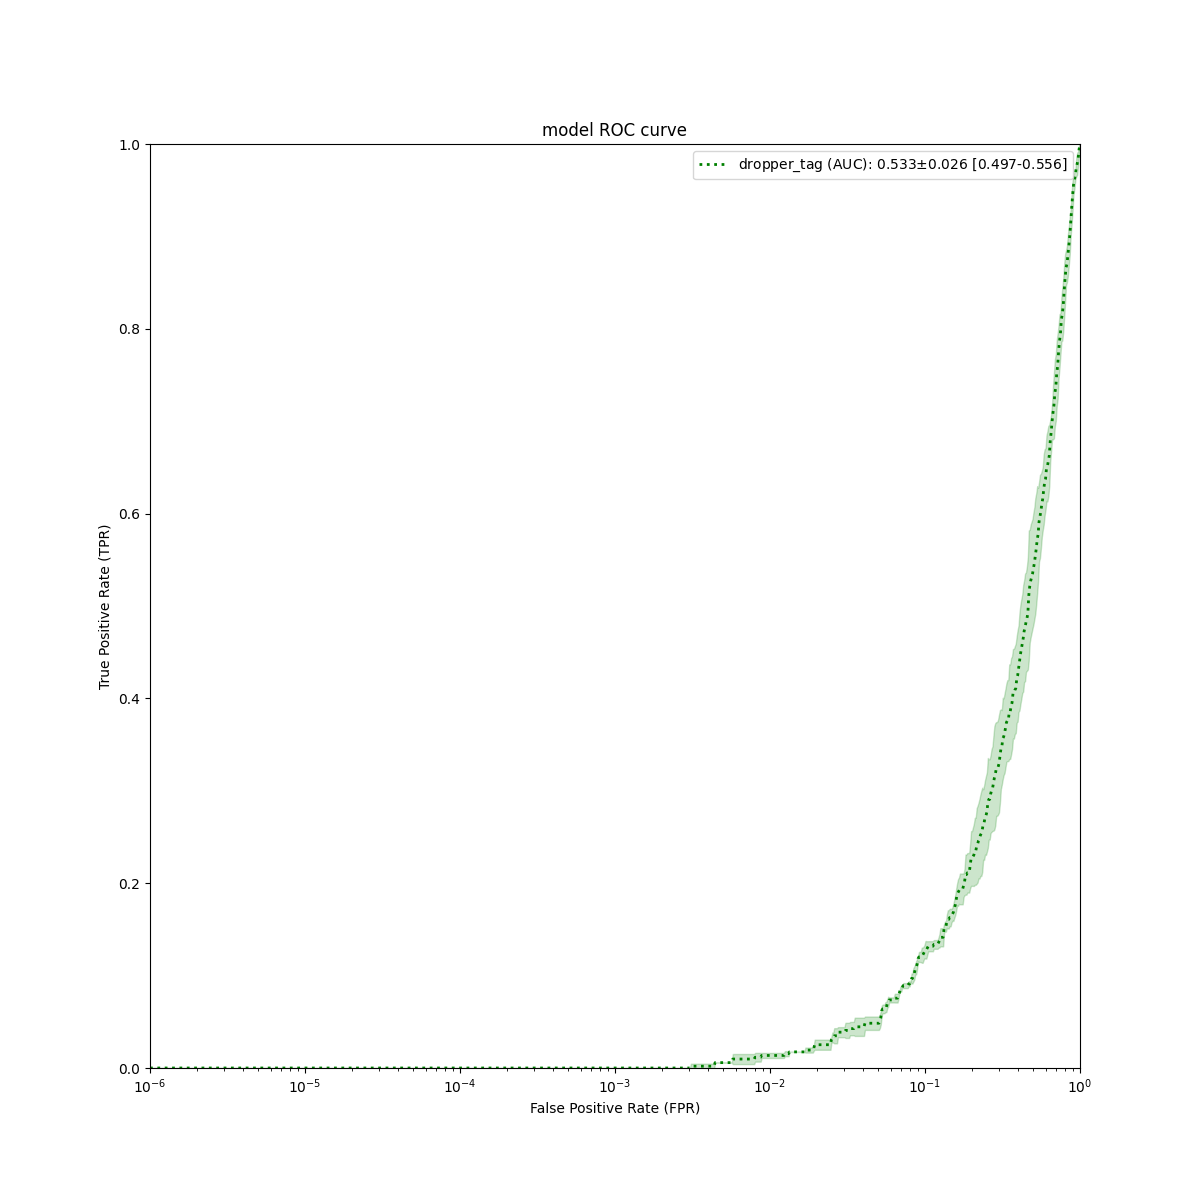
\includegraphics[width=0.6\textwidth]{./results/dropper_tag_roc_aloha.png}
        \vspace*{-0.2cm}
        \caption[Dropper Tag prediction task ALOHA ROC curve]{ROC curve and AUC statistics of \textBF{ALOHA} model for the \textbf{Dropper Tag}. The line represents the \textit{mean} TPR at a given FPR, while the shaded region represents the \textit{standard deviation}. Statistics were computed over \textBF{2} training runs, each with random parameter initialization.}
        \label{fig:dropperTagRocAloha}
    \end{figure}
}

\newcommand{\dropperTagRocProposedMethod}{
    \begin{figure}[H]
        \vspace*{-0.5cm}
        \centering
        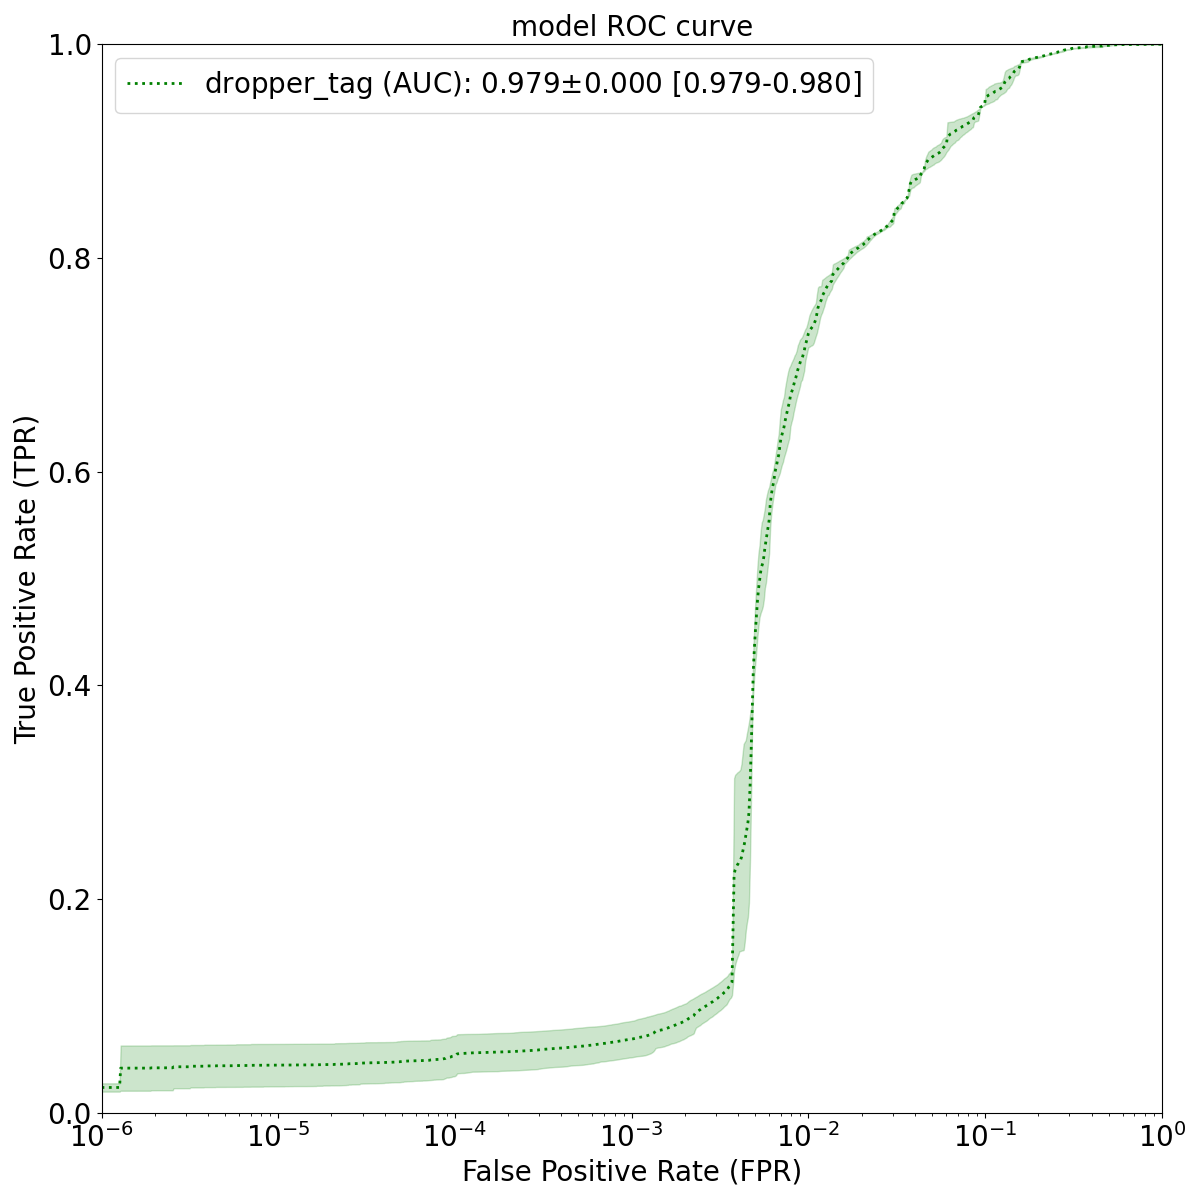
\includegraphics[width=0.6\textwidth]{./results/dropper_tag_roc_proposedModel.png}
        \vspace*{-0.2cm}
        \caption[Dropper Tag prediction task Proposed Model ROC curve]{ROC curve and AUC statistics of \textBF{Proposed Model} for the \textbf{Dropper Tag}. The line represents the \textit{mean} TPR at a given FPR, while the shaded region represents the \textit{standard deviation}. Statistics were computed over \textBF{2} training runs, each with random parameter initialization.}
        \label{fig:dropperTagRocProposedModel}
    \end{figure}
}
